
\begin{enumerate}
\item  
\question{Calculate the amount of current flowing through each element of the circuit in Figure~\ref{figSimpleComparatorCircuit}.  You can presume that the LM393 uses about $1\mymamp$ for its own (internal) operation, and that the LED is a red, $1.8\myvolt$ LED.  What is the total amount of current used by the circuit?}
\solution{$9.4\mymamp$}
\explanation{Let's start by analyzing the voltage divider created by R1 and R2.  
It connects directly to the positive and ground on the battery, so we know the total voltage across the divider ($9\myvolt$).
The operation of the LM393 utilizes negligible amounts of current, so we can ignore the amount of current coming out of the voltage divider to the LM393.  
The resistors are in series, so their resistance adds up to $1,000 + 1,000 = 2,000\myohm$.  
Therefore, we can find the current with Ohm's Law:
\begin{align*}
I &= V / R \\
  &= 9 / 2,000 \\
  &= 0.0045 \myamp = 4.5\mymamp
\end{align*}
The second voltage divider is similar, but has a total resistance of $2,000 + 4,000 = 6,000\myohm$.
Therefore, the current going across this voltage divider is:
\begin{align*}
I &= V / R \\
  &= 9 / 6,000 \\
  &= 0.0015\myamp = 1.5\mymamp
\end{align*}
The voltage coming into \icode{1IN+} is greater than the voltage coming into \icode{1IN-}, so that means that the LM393 output is positive.
When the output is positive, it actually disconnects (when it is negative, \icode{1OUT} connects to directly to ground).
Therefore, no current flows into \icode{1OUT}.

This allows all of the current to flow through the LED.
The LED utilizes $1.8\myvolt$, leaving $9 - 1.8 = 7.2\myvolt$ remaining for the resistor.
The resistor is $3,000\myohm$, so the current flowing through this part of the circuit is:
\begin{align*}
I &= V / R \\
  &= 7.2 / 3,000 \\
  &= 0.0024 \myamp = 2.4\mymamp
\end{align*}
Therefore, the first voltage divider is using $4.5\mymamp$, the second voltage divider is using $1.5\mymamp$, the LED circuit is using $2.4\mymamp$, and the internal operation of the LM393 uses $1\mymamp$ (per the problem statement).
Therefore, the total current used by this circuit is $4.5 + 1.5 + 2.4 + 1 = 9.4\mymamp$.
}
\item 
\question{Take the circuit in Figure~\ref{figSimpleComparatorCircuit} and swap which voltage divider is attached to \icode{1IN+} and \icode{1IN-}.  Now calculate the total amount of current used by this circuit.}
\solution{$10\mymamp$}
\explanation{If the inputs to the LM393 are swapped, this would not change the current usage of the voltage dividers, or the internal operation of the LM393.
However, in this configuration, the output (\icode{1OUT}) is negative.
In the case of the LM393, this connects the output to ground.

Therefore, the LED will not light up because the voltage will get to zero before it hits the LED.
Thus, the voltage across R5 will be the entirety of the $9\myvolt$.
Therefore, the new current calculation will be:
\begin{align*}
I &= V / R \\
  &= 9 / 3,000 \\
  &= 0.003\myamp = 3\mymamp
\end{align*}
Therefore, using the results from the previous question, we can see that the total current usage is $4.5 + 1.5 + 3 + 1 = 10\mymamp$.
}
\item 
\question{The Spectra Flex Sensor is a resistive sensor that changes its resistance when bent.  When it is straight, it has a resistance of $10\mykohm$.  When it is bent, it has resistances of $60\mykohm$ and above.  Draw a circuit that turns on an LED when the resistor is bent.  Use a resistor symbole for the flex sensor, but label it as \icode{FLEX}.}
\solution{}
\explanation{You can create a circuit to do this using the same voltage comparator circuit as before, but with one of the voltage dividers replaced with the circuit shown:
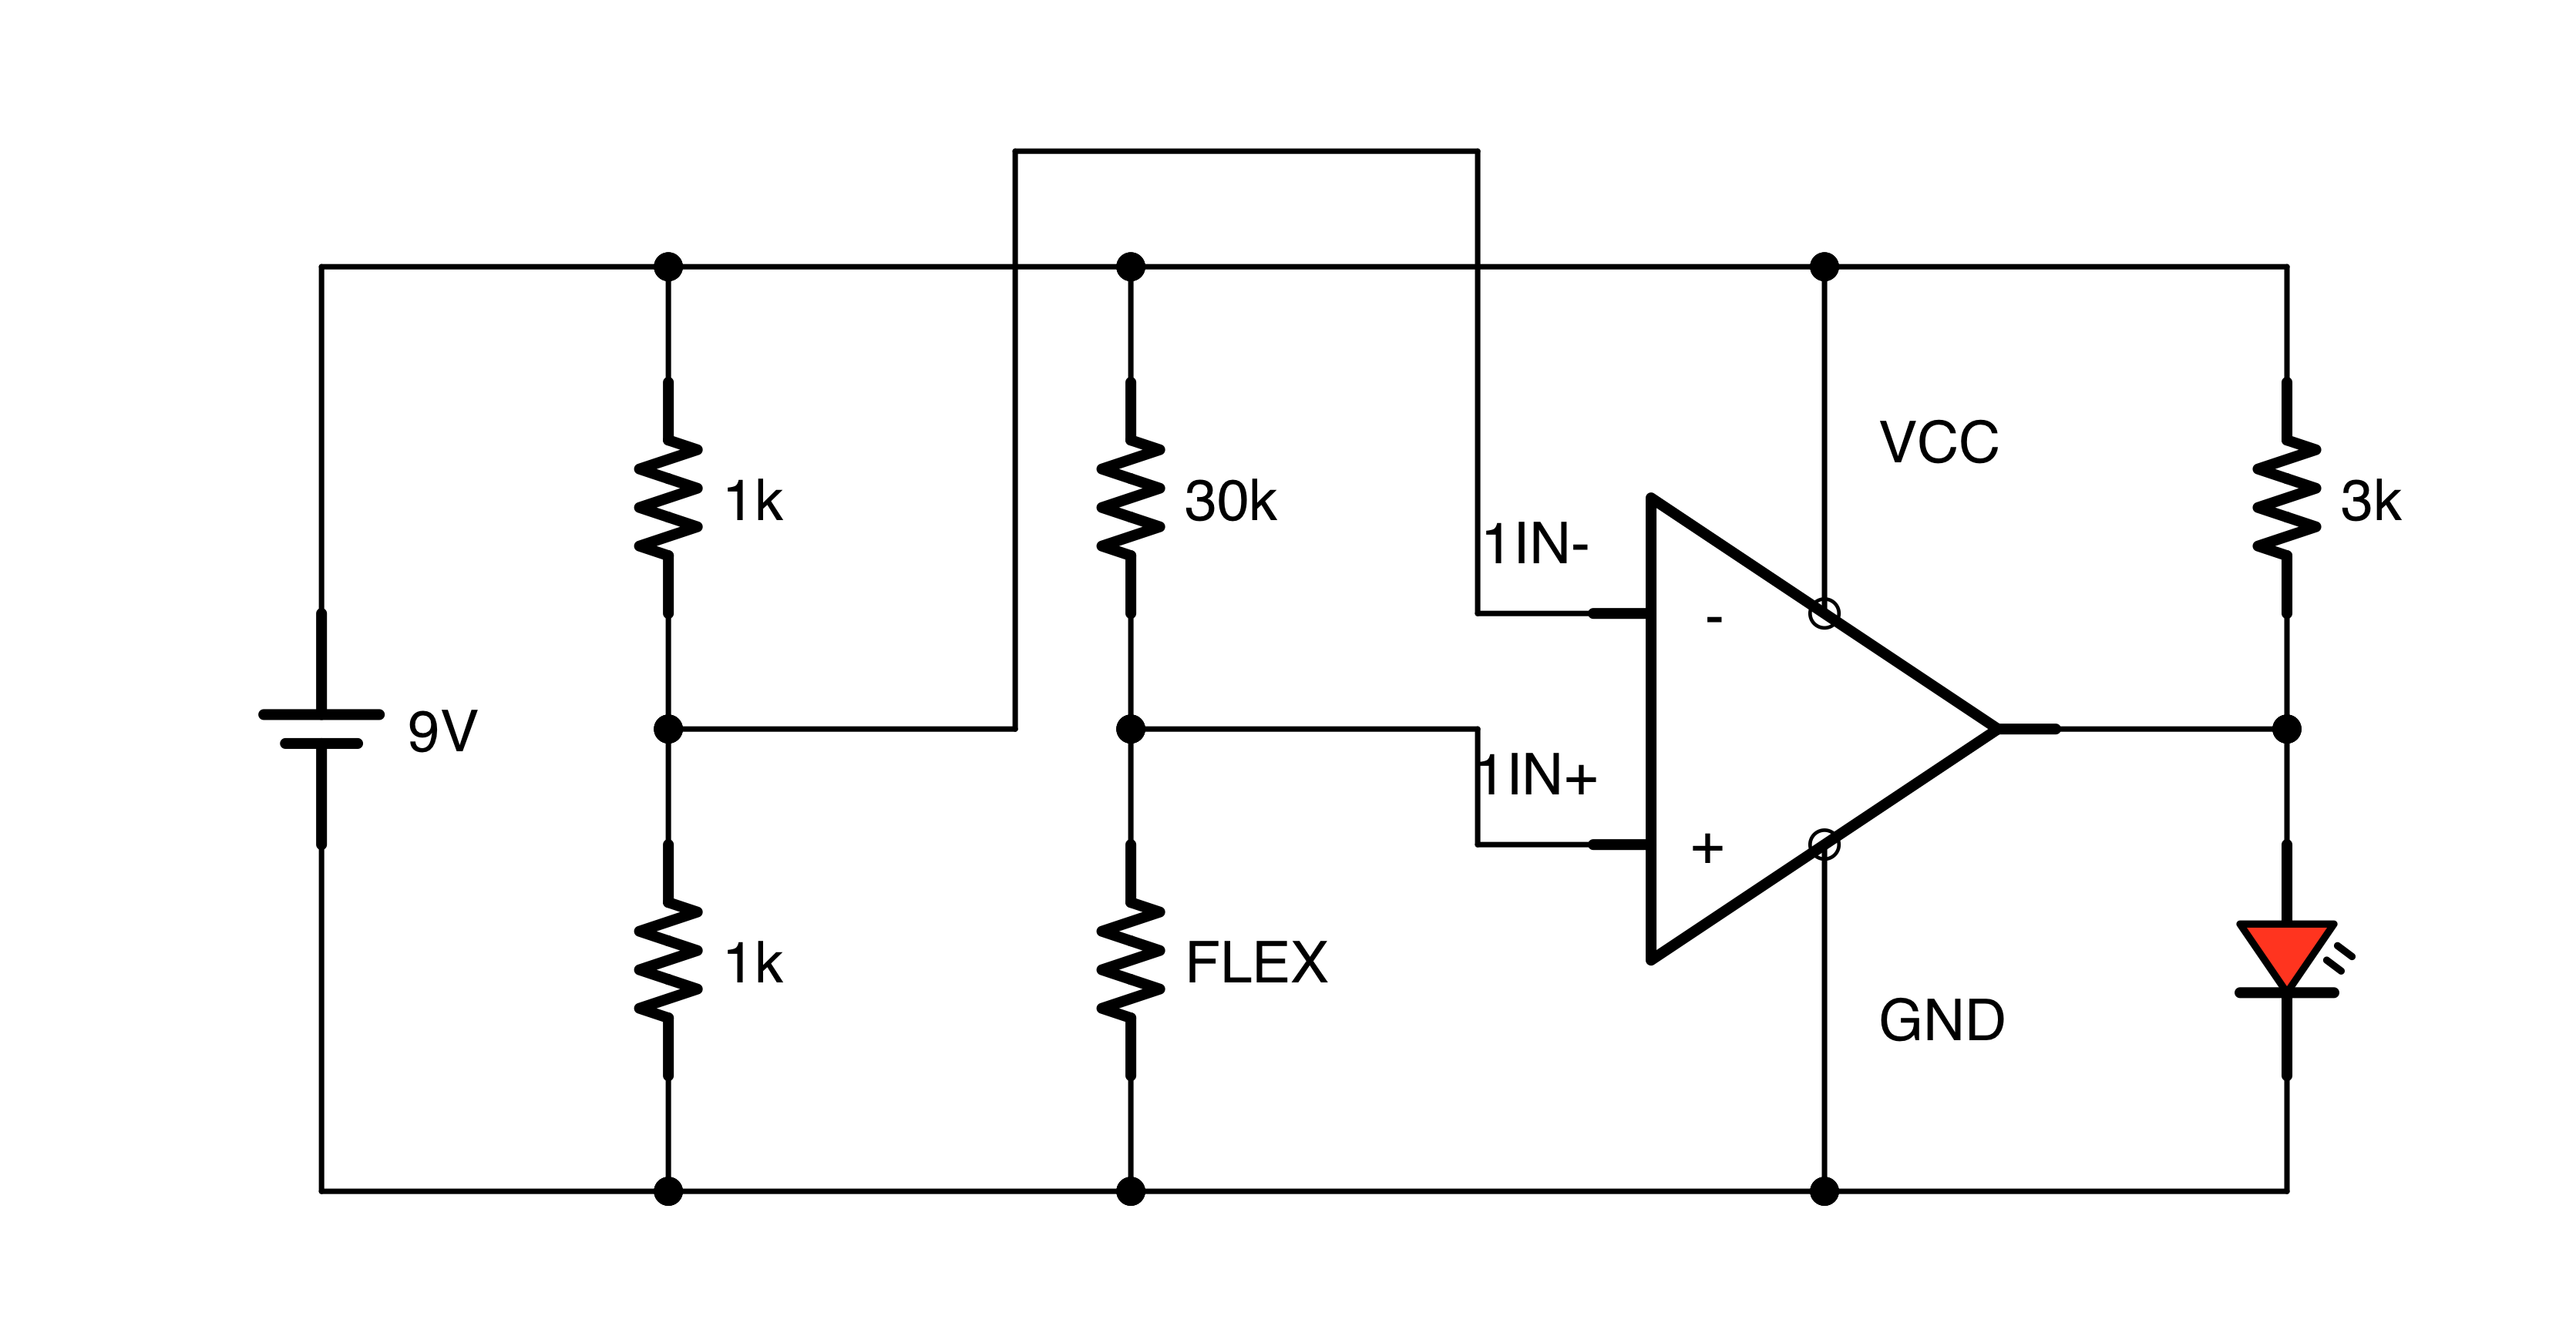
\includegraphics[width=\columnwidth]{ExFlexSensor.png}
In this circuit, when the Flex sensor is straight, the middle voltage divider will go lower than the divider on the left, turning the output negative (i.e., connecting it to ground).
When the Flex sensor is bent, the middle voltage divider will go higher than the divider on the left, turning the output positive (i.e., disconnecting the output from the circuit and allowing the current to flow through the LED).
Thus, putting a variable resistor as part of a voltage divider will convert the changing resistance into a changing voltage.

The actual values of the resistor do not matter nearly as much as their ratios.
On the left divider, it only matters that the resistors are equal (so the voltage is divided in half).
On the middle divider, it only matters that the non-Flex resistor value is \emph{between} the straight and the bent resistance, so that as it goes between straight and bent the voltage will swing above and below the voltage of the left voltage divider.
}
\item 
\question{Build the circuit in Figures~\ref{figDarknessSensorCircuit} and~\ref{figDarknessSensorBreadboard}.}
\solution{On this circuit, be sure to test it in a variety of light levels.}
\item 
\question{If you wanted to wait until the room was even darker before the LED went on, how would you change the circuit?}
\solution{The photoresistor works by increasing resistance in the dark.  If you increase the resistance of R3, then you increase the amount of darkness required to move the voltage above the reference voltage from the other voltage divider and activate the circuit.}
\end{enumerate}
